\documentclass[a4paper,11pt,oneside,fleqn]{article}
% Pakker
\usepackage[utf8]{inputenc} % Så må vi bruge æ, ø og å
%\usepackage[ansinew]{inputenc}
%\usepackage[danish]{babel} % Dansk opsætning
\usepackage[T1]{fontenc} % Hjælper med ordeling ved æ, ø og å. Sætter fontene til at være ps-fonte i stedet for bmp.
\usepackage[english,final]{varioref} % Vi kan anvende \vref
\usepackage{array,booktabs} % Til gode tabeller
\usepackage{acronym} % Smart akronymhåndtering
\usepackage{minitoc} % Vi kan lave del inholdsfortegnelser forhåbentlig
\usepackage{graphicx} % We can now use \includegraphics and stuff
\usepackage{pdfpages} % Inkludere en pdf side som en side  
\usepackage{bytefield}


\begin{document}
\author{Nick Østergaard \and Rasmus Lundgaard Christensen \and Frederik Juul \and Attila Frodor \and Todor Muresan}
\title{Worksheet \#1 by group 12gr730}
\date{\today}
\maketitle

\section{Introduction}
Measuring the waters around Greenland (or any watery nation in particular) is a a time consuming task. Today, these measurements are carried out by large vessels that sail up and down along the coastline, and into the many fjords as well. These vessels require alot of man power to operate, and are thereby quite expensive to run.

The purposes of these measurements is to measure the water depth, so that larger ships can take short routes to reach their destination, and for geographers to map areas which they previously found too expensive. Another important fact about the mapping, is that an increase in the cruise ships that sail to Greenland has increased. A sinking cruise ship will cause many problems, not only to the nature, but also to Greenland itself. The infrastructure of Greenland is not capable of handling a sudden increase of population of 5-10\%, so developing a smarter way of mapping the waters could pose a solution suitable for all implicated parts. 

As stated, when measuring water depths today, a ship is sailing out into the water, holding still whilst measuring the time difference using an echo sounder, and then saves this position and depth. This particular task can however be done by smaller vessels that in turn could be made fully autonomous, thus making the mapping cheap whilst still really efficient (as autnonomous vessels wouldn't need to sleep). 

Such a vessel would be under the influence of disturbances such as wind, waves and the current, making it hard to stay still in the same position to obtain an actual measurement. The speed of sound in water is about 1484 m/s and if the beam is not shot perpindicular to the surface, the angle might be so that the vessel will not be able to read the returned sound beam. 

\begin{figure}[h]
\centering
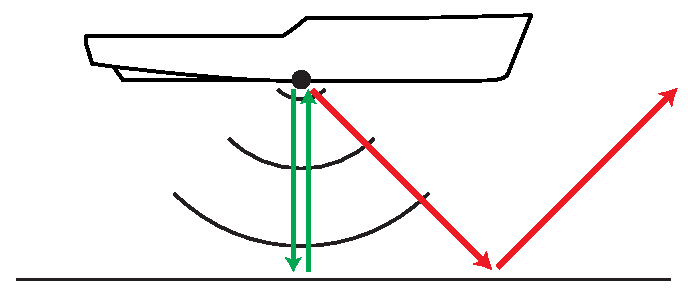
\includegraphics[width=0.5\textwidth]{img/beamer}
\caption{Overview of a depth mapping system}
\label{fig:beamer}
\end{figure}

This report will then describe the development of such an autonomous craft, that can be used for measuring the water depth whilst under the influence of external forces such as waves, wind and current. 

\end{document}